\documentclass[a4paper]{exam}
\usepackage{epsf}
\usepackage{hyperref}
\usepackage{url}
\usepackage{graphicx}
\usepackage{cite}
\usepackage[top=2cm,left=2cm,right=2cm]{geometry}
\usepackage{amsmath}
\usepackage[]{algorithm2e}
\usepackage[french]{babel}
\usepackage[utf8]{inputenc}
\usepackage{xcolor}
\DeclareMathOperator*{\argmin}{arg\,min}

\newtheorem{question}{{\bf Q.}}[section]

\title{TD 1 Apprentissage par Renforcement - Master AIC}

\author{Laurent Cetinsoy, Diviyan Kalainathan, Michèle Sebag}

\begin{document}

\maketitle

\section{Exercice de cours}

Ces questions ont pour but de vous aider à clarifier les différentes notions. Réponses courtes attendues.


\begin{question}

Quel est le but d'un algorithme d'un apprentissage par renforcement ? \em{what is the goal of Reinforcement Learning}

\end{question}


\begin{question}

Dans ce cadre quel est le but d'un agent ? \em{In this framework what is the goal of an agent}

\end{question}

\begin{question}
Comment le traduire formellement ? \em{How can you formalize it mathematically ?}

\end{question}

\begin{question}
	Qu'est ce qui différencie d'après vous un problème de RL d'un problème supervisé ? Qu'est ce qui rend un problème de RL Difficile ? \em{What make reinforcement learning different from supervised learning ? What makes reinforcement learning hard ?}
\end{question}

\begin{question}

Formellement, qu'est ce qu'un MDP ? Donnez la signification de ses composants. \em{Give the formal definition of a Markov Decision Process (MDP). Give the meaning of it components}

\end{question}

\begin{question}
	Que represente le taux d'actualisation (discount), souvent noté $\gamma$ ? \em{What does the discount factor $\gamma$ mean or represent ?}
\end{question}


\begin{question}
	Pouvez vous donner des exemples de problèmes où les transitions ne sont pas déterministes ? \em{Can you give exemples of setup With non deterministic transitions ?}
\end{question}

\begin{question}
	De quoi dépend la récompense R ? \em{On what depends the reward function R}
\end{question}

\begin{question}
 Pour les problèmes suivants indiquer si l'espace des actions et des états est continu ou discret : \em{For each setups, tells if the space of action and state are continuous or discrete}

 \begin{itemize}
 	\item{Cartpole. \em{Cartpole}} 
 	\item{La voiture autonome \em{Autonomous car}}
 	\item{Le poker. \em{Poker}}
 	\end{itemize}

\end{question}


\begin{question}
Quelle est la différence entre un problème épisodique et continue ? Donner un exemple de chaque. \em{What is the difference of an episodic setup and a continuous one ? Give an example of each}
\end{question}

\begin{question}
Que réprésentent / signifient les fonctions de valeur V et Q ? \em{What does the V and Q functions means or represents ?}
\end{question}

\section{Exercice du labyrinthe}

On considère un agent dans le labyrinthe ci dessous qui contient 27 cases. \em{Let us consider the following labyrinth made of 27 white boxes}

\begin{figure}[h]
	\begin{center}
		\includegraphics*[height=6cm]{maze.png}
	\end{center}
\end{figure}


Afin de lui apprendre à chercher la sortie, on lui donne une récompense de +r quand il est dans la case de sortie (Goal) et une punition de moins $-\alpha r$ à chaque fois qu'il se trouve dans une autre case. On considère cet l'environement déterministe : si l'agent décide d'aller à une case blanche adjacente, il se retrouve bien à cette case.

\em{In order to teach him to find to reach the exit, we give it a positive reward +r if is reach the goal and and punition of $-\alpha r$ each time he is on another white square. We consider the environment as deterministic: if the agent decides to go to an adjacent white box, it indeed goes there.}

\begin{question}
	Quel est l'espace des états ? \em{What is the space of states ?}
\end{question}

\begin{question}
	Quel est l'espace des actions ? \em{What is the space of actions ?}
\end{question}

\begin{question}
	Pourquoi met-on on un reward négative à chaque itération qui n'atteint pas l'objectif ? \em{Why do we give a negative reward when the agent does not reach the goal ?}
\end{question}


\begin{question}
Donner l'équation de bellman vérifiée par V \em{Give the bellman equation folloWed by V}
\end{question}

\begin{question}
En déduire V pour chacun des états pour la politique optimale (c'est à dire si à chaque état, l'agent prend la meilleur décision possible). \em{Deduce what is V for each state for the optimal policy (the one where the agent takes the best decision at each step)}

\end{question}

\section{Grille}

On considère l'environement suivant: un agent peut se déplacer sur une grille dans les quatre direction de l'espace (sauf quand il se retrouve au bord). Quand il se retrouve en A, l'agent reçoit une récompense de +10 et se retrouve téléporté en A'. Quand l'agent se trouve en B, il reçoit une récompense de +5 et se retrouve téléporté en B.

\em{Let us consider the following environment: an agent can move a 2D grid in the four dimensions (except when it reaches the border). when it is on A, it receives a +10 reward and is teleported to A'. when it is in B, it receives a +5 reward and is teleported to B'}

\begin{figure}[h]
	\begin{center}
		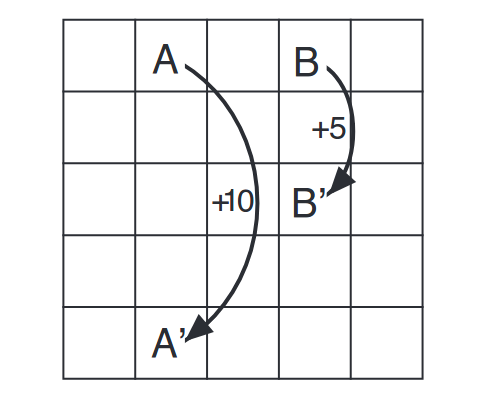
\includegraphics[height=6cm]{grille.png}
	\end{center}
\end{figure}


\begin{question}

On considère la politique explicite suivante: Toujours aller vers le haut. Estimer la fonction de valeur pour chacun des états. On considère un horizon infini et on prendra pour facteur d'actualisation $\gamma = 0.9$. \em{We consider the following policy: always going upside. Give the value function for all states. We consider an infinite horizon and we will take $\gamma=0.9$ as discount factor.}

\end{question}

\begin{question}
	S'agit-il de la meilleur politique possible ? Dans le cas contraire proposer la meilleur. \em{Is it the best policy one can find ? If not give the best one}
\end{question}

\section{Rivière}

On souhaite faire traverser une rivière à un agent que l'on représente par N cases. La case une est le versant de départ, la case N le versant d'arrivé. L'espace des état est donc {1..N} et l'espace des action est {gauche, droite}. La fonction de récompense est la suivante : R(s) = 0 pour $s < N$ et R(N) = 100. L'état N est terminal. Le facteur d'escompte est $\gamma = .9$.

\em{we want to make an agent cross a river modelised by N boxes. The box number 1 is the starting point and the box N is the goal. The state space is thus {1..N} and the action space is {left, right} the reward function if R(s) = 0 for $s < N$ and R(N) = 100. State N is terminal. Discount factor $\gamma = 0.9 $}

\centerline{\setlength{\unitlength}{2144sp}%
%
\begingroup\makeatletter\ifx\SetFigFont\undefined%
\gdef\SetFigFont#1#2#3#4#5{%
  \reset@font\fontsize{#1}{#2pt}%
  \fontfamily{#3}\fontseries{#4}\fontshape{#5}%
  \selectfont}%
\fi\endgroup%
\begin{picture}(11274,1377)(889,-2776)
\thinlines
{\color[rgb]{0,0,0}\put(901,-2311){\framebox(900,900){}}
}%
{\color[rgb]{0,0,0}\put(2251,-2311){\framebox(900,900){}}
}%
{\color[rgb]{0,0,0}\put(3601,-2311){\framebox(900,900){}}
}%
{\color[rgb]{0,0,0}\put(4951,-2311){\framebox(900,900){}}
}%
{\color[rgb]{0,0,0}\put(11251,-2311){\framebox(900,900){}}
}%
\put(2701,-2761){\makebox(0,0)[lb]{\smash{{\SetFigFont{20}{24.0}{\rmdefault}{\mddefault}{\updefault}{\color[rgb]{0,0,0}2}%
}}}}
\put(4051,-2761){\makebox(0,0)[lb]{\smash{{\SetFigFont{20}{24.0}{\rmdefault}{\mddefault}{\updefault}{\color[rgb]{0,0,0}3}%
}}}}
\put(5401,-2761){\makebox(0,0)[lb]{\smash{{\SetFigFont{20}{24.0}{\rmdefault}{\mddefault}{\updefault}{\color[rgb]{0,0,0}4}%
}}}}
\put(11701,-2761){\makebox(0,0)[lb]{\smash{{\SetFigFont{20}{24.0}{\rmdefault}{\mddefault}{\updefault}{\color[rgb]{0,0,0}N}%
}}}}
\put(1351,-2761){\makebox(0,0)[lb]{\smash{{\SetFigFont{20}{24.0}{\rmdefault}{\mddefault}{\updefault}{\color[rgb]{0,0,0}1}%
}}}}
\put(7201,-1861){\makebox(0,0)[lb]{\smash{{\SetFigFont{20}{24.0}{\rmdefault}{\mddefault}{\updefault}{\color[rgb]{0,0,0}....}%
}}}}
\put(8551,-1861){\makebox(0,0)[lb]{\smash{{\SetFigFont{20}{24.0}{\rmdefault}{\mddefault}{\updefault}{\color[rgb]{0,0,0}....}%
}}}}
\put(9901,-1861){\makebox(0,0)[lb]{\smash{{\SetFigFont{20}{24.0}{\rmdefault}{\mddefault}{\updefault}{\color[rgb]{0,0,0}....}%
}}}}
\end{picture}%

}

\begin{question}
	Let $\pi$ be a random policy ($\pi(s) = Left$ or $Right$ with probability 1/2). Let the transition function be defined as:
	\[ \begin{array}{lll}
	p(i,Right,i+1) = 1 & \mbox{~if~ } i < N \\
	p(i,Left,i-1) = 1 & \mbox{~if } i > 0 & \mbox{~else~} p(0,Left,0) = 1 \
	\end{array} \]
	What is the probability of arriving in state $N$ after 100 time steps ? After 1,000 time steps ?\\
	{\em Soit $\pi$ une politique al\'eatoire ($\pi(s) = Left$ ou $Right$ avec probabilit\'e 1/2). Avec la fonction de transition ci-dessus, quelle est la probabilité d'arriver à l'état $N$ en 100 pas de temps ? en 1,000 pas de temps ?}

\end{question}

\begin{question}
	Let $\pi$ be the constant policy, $\pi(s) = Right$ for all $s$. With same function transition as above, compute the value function (function of $N$).\\
	{\em Soit $\pi$ la politique constante qui va toujours à droite. Avec la meme fonction de transition que pour la question précédente, calculez la fonction de valeur associée à $\pi$ (fonction de $N$).}
\end{question}

\begin{question}
	Same question with $p(i,Right,i+1) = .9; ~p(i,Right,i) = .1$.\\
	{\em Même question avec une fonction de transition probabiliste, $p(i,Right,i+1) = .9; ~p(i,Right,i) = .1$.}
\end{question}

\section{Pole balancing}

On considère le problème de maintenir en équilibre un baton tenu par sa base à chariot pouvant se déplacer. Let us consider the CartPole problem where on wants to maintain a stick vertically. The stick is fixed at the bottom to a cartpole that can move.


\begin{figure}[h]
	\begin{center}
		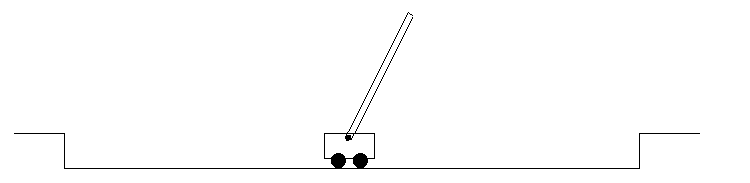
\includegraphics[width=15cm]{pole-balancing.png}
	\end{center}
\end{figure}

\begin{question}
	Proposez une structure de reward qui permettrait aux algorithmes de RL à apprendre à garder en équilibre la barre. \em{Propose a reward structure which would likely induce the desired behavior}
\end{question}

\begin{question}
	Étant donné une Q function définie, comment peut-on choisir la prochaine action ; cad comment à partir de Q obtient on la policy ? Voyez-vous un problème à cette approche ? \em{Given a Q function, how one could use it to choose the next action to perform? Can you see a problem to this approach ?}
\end{question}

\end{document}
